\documentclass[11pt, oneside]{article}   	% use "amsart" instead of "article" for AMSLaTeX format
\usepackage[margin=0.7in]{geometry}                		% See geometry.pdf to learn the layout options. There are lots.
\geometry{letterpaper}                   		% ... or a4paper or a5paper or ... 
%\geometry{landscape}                		% Activate for rotated page geometry
%\usepackage[parfill]{parskip}    		% Activate to begin paragraphs with an empty line rather than an indent
\usepackage{graphicx}				% Use pdf, png, jpg, or eps§ with pdflatex; use eps in DVI mode
								% TeX will automatically convert eps --> pdf in pdflatex		
\usepackage{amssymb}
\usepackage{amsmath}
\usepackage{amsfonts}
\usepackage{listings}
\usepackage{dsfont}
\usepackage{wasysym}

%SetFonts

%SetFonts


\title{Oscillations in the Oxide-fuelled ABR ULOF with ARC System Implementation}
\author{Chris Keckler}
%\date{}							% Activate to display a given date or no date

\begin{document}
\maketitle

With the optimal ARC system chosen for the oxide-fuelled ABR core \cite{2017ANSWinter_ARC}, short coolant and cladding temperature oscillations are present within the early phase of the ULOF transient.
The purpose of this report is to investigate the cause and impact of these oscillations, and to gather information useful towards the design of future ARC systems.

%%%%%%%%%%%%%%%%%%%%%%%%%%%%%%%%%%%%%%%%%%%%%%%%%%%%%%%%%%%%%%%%%%%%%%%
\section{Nature of the oscillations}

Two sets of oscillations are seen in the ULOF accident sequence with the ARC system installed -- each are of a different nature.
One set of oscillations are caused by the transition from forced to natural circulation and occur in the ULOF sequence regardless of if an ARC system is installed or not.
The other set of oscillations are induced by the ARC system actuation in response to the rapidly changing coolant temperatures during the early phase of the ULOF sequence.
Both of these oscillation types are outlined below.

%%%%%%%%%%%%%%%%%%%%%%%%%%%%%%%%%%%%
\subsection{Oscillations induced by the transition from forced to natural circulation} \label{flowInduced}

The ULOF accident is characterized by a rapid decrease in coolant flowrate during the very early phase of the accident.
As the pump coasts down, the flow rate continuously halves according to the pump halving time (20 s for this core design) until reaching a pump impeller speed at which the rotor locks due to insufficient rotational momentum.
Upon rotor locking, the flow rate makes a sudden transition from a low-flow forced circulation to the natural circulation rate appropriate for the power level.
In response to the sudden transition while the reactor is still at substantial power (often above 10\%), the coolant heats up rapidly due to the power/flow mismatch, leading to a prompt increase in fuel and cladding temperatures.
This temperature increase causes a strong negative reactivity insertion from the doppler, axial expansion, radial expansion, and CRDL feedbacks, which then causes the power to rapidly decrease and for temperatures to rapidly drop back down. 
This sequence of rapid temperature changes spurs a set of temperature/power oscillations which eventually damp out as the reactor approaches its equilibrium state.
Figure \ref{fig:nominalULOF} shows the response described above for the case of a ULOF in the nominal oxide ABR core (no ARC system implemented), where the oscillations begin at about 700 s.

\begin{figure}[h!]
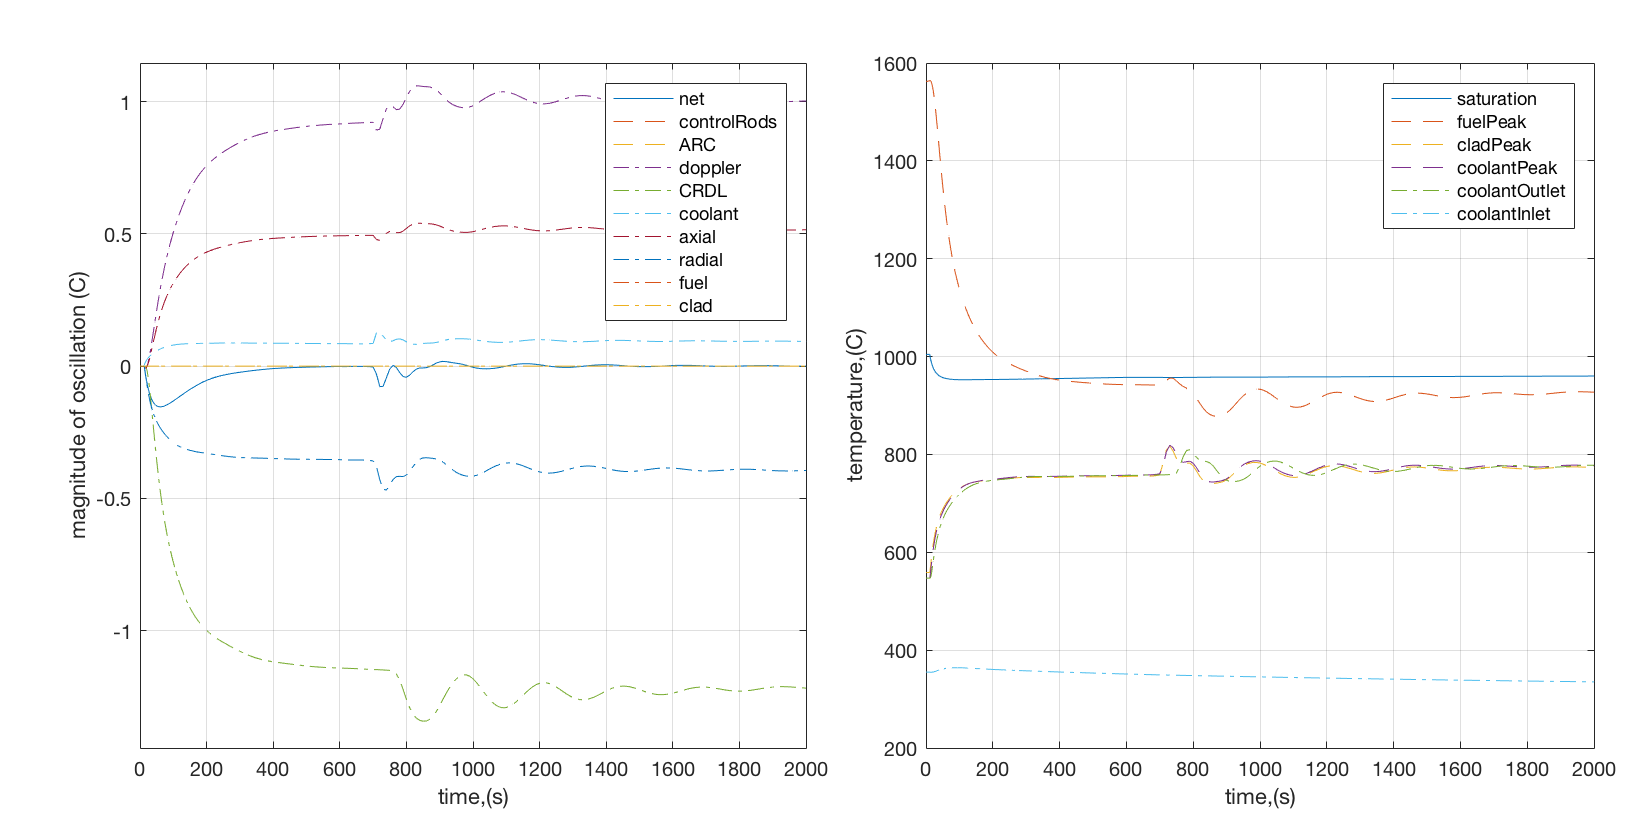
\includegraphics[width=18cm]{nominalULOF}
\centering
\caption{Response to a ULOF accident in the nominal oxide ABR core.}
\label{fig:nominalULOF}
\end{figure}

The oscillations seen during this transition phase are relatively slow, with around 200 s from crest-to-crest. 
However, the magnitude of the oscillations is relatively large immediately following the flow transition, with peak-to-valley magnitudes of around 60 C.
Combining these aspects gives a temperature ramp rate of 1.76 C/s. 
The sequence of oscillations persists for nearly 2000 s (33 minutes), although the oscillation magnitude drops off sharply after the first few peaks. 
Although these oscillations are undesirable, they occur at a low power level, and thus do not bring the coolant close to boiling or the clad/fuel close to melting, making them mostly benign.

Another noteworthy aspect of these oscillations is that they are largely unimpacted by the presence of an ARC system in the core. 
To demonstrate this, Figure \ref{fig:ULOF_oscillationsWithS} shows the peak-to-valley magnitude of the oscillations following the transition from forced to natural circulation for increasing values of the actuation span, $S$, of an ARC system with an actuation temperature of 10 C and a total worth of \$0.87.
From the flat trend, it is clear that the oscillations induced by the flow transition are not impacted by the ARC system span.
A similar trend is seen with all other ARC system design variables as they relate to the oscillations caused by the flow transition.

\begin{figure}[h!]
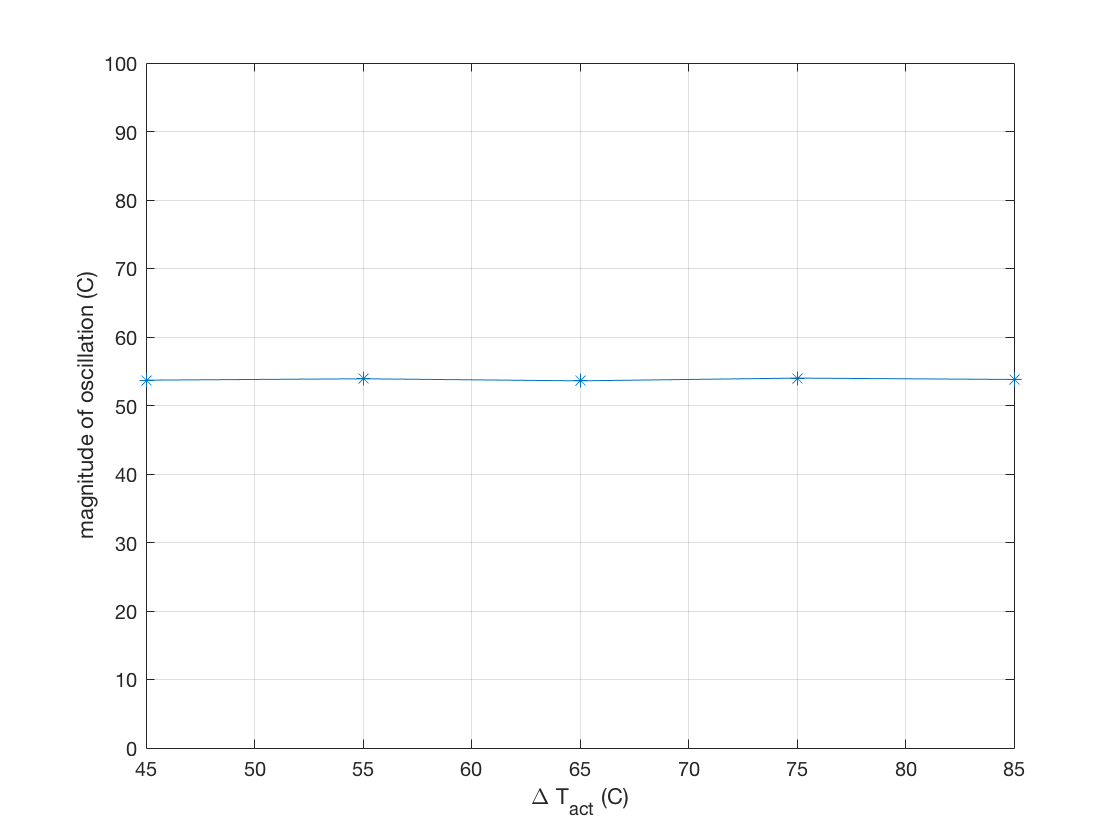
\includegraphics[width=10cm]{ULOF_oscillationsWithS}
\centering
\caption{Peak-to-valley magnitude of outlet coolant temperature oscillations following the transition from forced to natural circulation in the oxide ABR equipped with an ARC system with $\Delta T_{act} = 10$ C and $w = \$0.87$.}
\label{fig:ULOF_oscillationsWithS}
\end{figure}

The reason for this insensitivity is clear when examining the reactivity response of the core with an ARC system equipped, as shown in Figure \ref{fig:ULOF_65_0.87_10}.
By the time that the flow-transition-induced oscillations occur at near 700 s, the coolant temperature is already at 655 C, which is more than 100 C above the nominal coolant temperature. 
Because the ARC system is actuated at only 10 C and then it takes only an additional 65 C for the lithium absorber to reach full actuation, the ARC system is already fully actuated by the time the oscillations occur. 
For all examined ARC system designs in which boiling is not seen to occur during the transients, the ARC system is not able to improve the behavior of the flow-transition-induced oscillations for this same reason.
In many ARC designs which would allow for the system to be only partially actuated at these coolant temperatures (i.e. when $S+\Delta T_{act} > 100$), the sluggish response of the ARC system causes boiling to occur from growing oscillations that form during the early ULOF transient phase.
Additionally, in the designs examined where the ARC system was not fully actuated at the time of the flow transition, the ARC system was mostly actuated, and the remaining reactivity insertion was weak due to the S-shaped incremental worth curve for the ARC system.
Therefore, it is possible that the ARC system could provide benefits to this type of oscillation if the flow transition occurred earlier in the transient when the coolant temperatures are lower, but no benefits are seen specifically for the oxide ABR core.

\begin{figure}[h!]
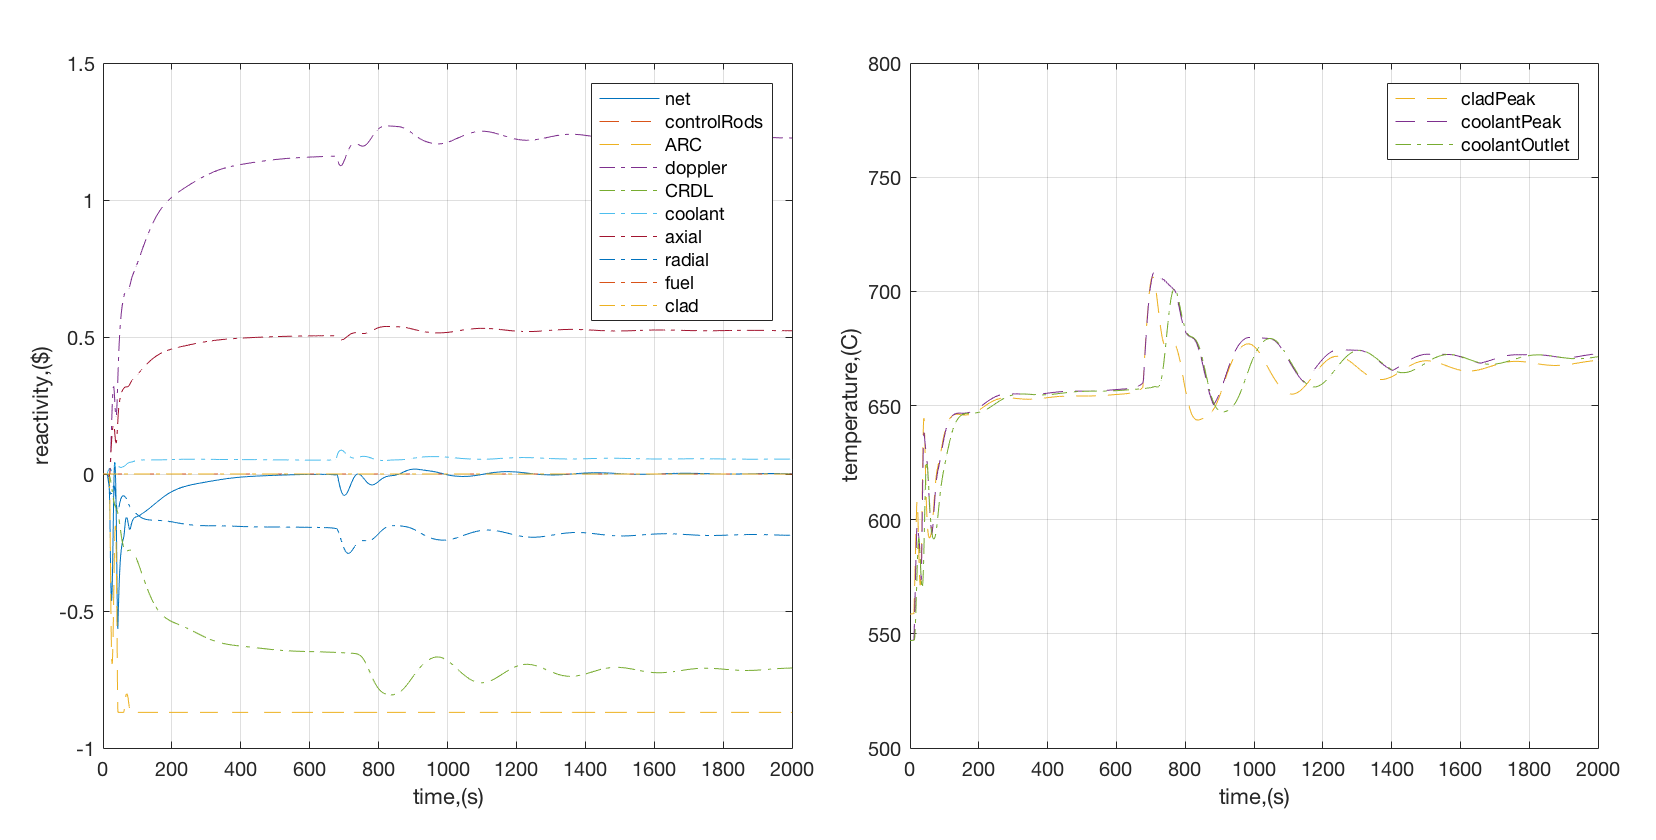
\includegraphics[width=18cm]{ULOF_65_087_10}
\centering
\caption{Transient response to a ULOF accident in the oxide ABR equipped with an ARC system of $S=65$ C, $w=\$0.87$, and $\Delta T_{act} = 10$ C.}
\label{fig:ULOF_65_0.87_10}
\end{figure}

%%%%%%%%%%%%%%%%%%%%%%%%%%%%%%%%%%%%
\subsection{ARC system induced oscillations} \label{sec:increasingS}

The other type of oscillations that are seen to occur in the ULOF transient with the optimal ARC system installed happen during the early phase of the transient, when the flow is rapidly dropping off.
An example of these oscillations are shown in Figure \ref{fig:ULOF_65_0.87_10_early} for the oxide ABR core with the optimal ARC design of $S=65$ C, $w=\$0.87$, and $\Delta T_{act} = 10$ C.
It is seen that the coolant and clad temperatures both suffer from oscillations of around 30 C.
Although these oscillations are of smaller magnitude than those induced by the flow transition described above, they are more rapid, leading to a similar temperature ramp rate. 

\begin{figure}[h!]
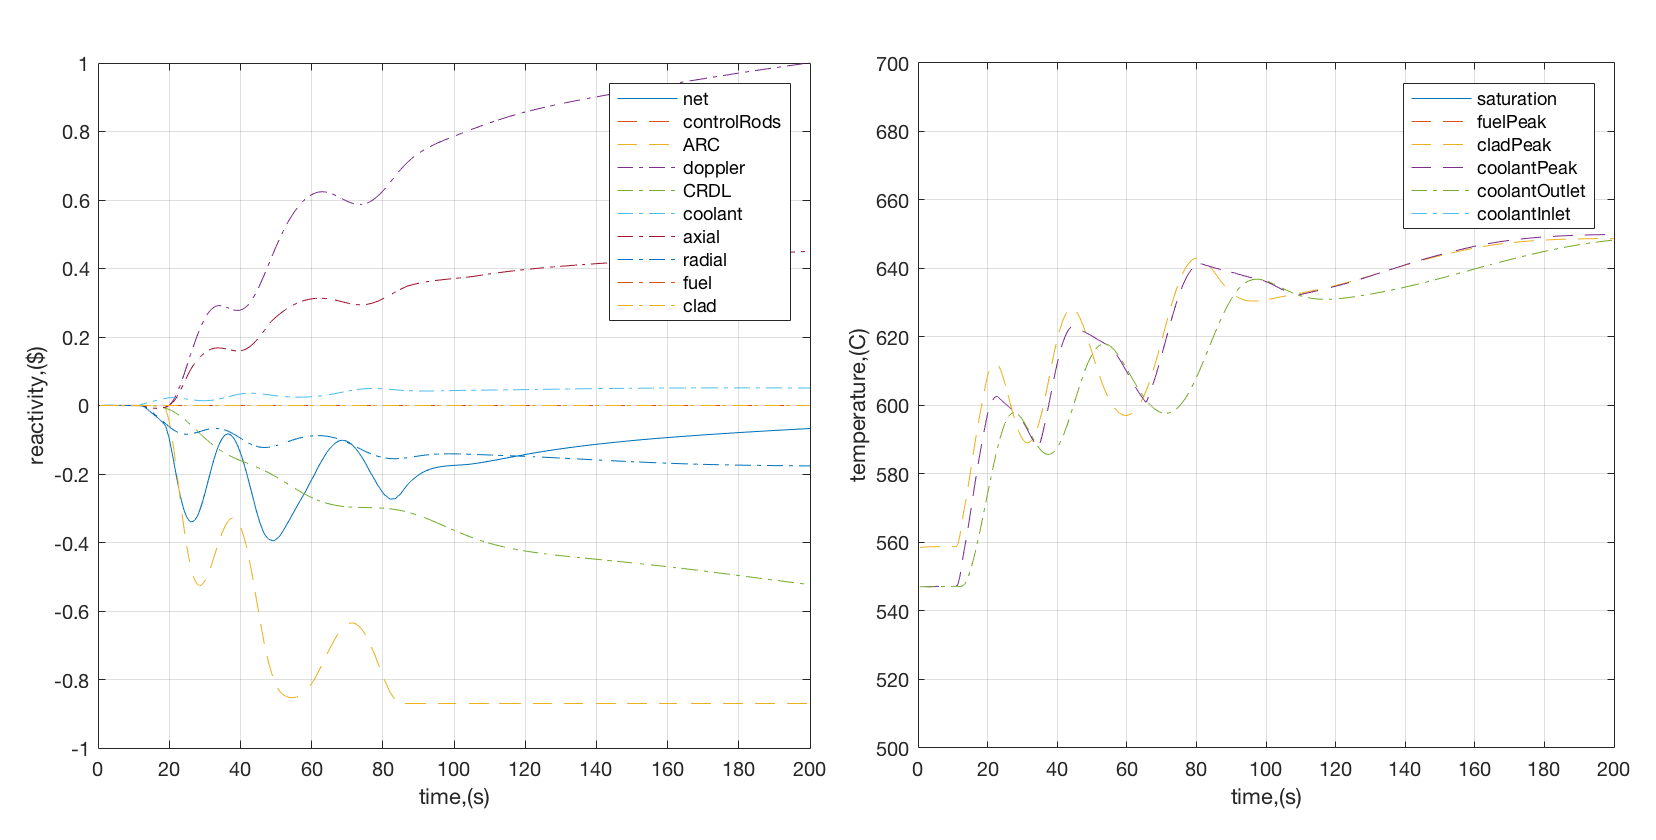
\includegraphics[width=18cm]{ULOF_65_087_10_early}
\centering
\caption{Transient response during the early phase of a ULOF accident in the oxide ABR equipped with an ARC system of $S=65$ C, $w=\$0.87$, and $\Delta T_{act} = 10$ C.}
\label{fig:ULOF_65_0.87_10_early}
\end{figure}

An aspect of these oscillations that is much different from those outlined in Section \ref{flowInduced}, however, is how they die out.
The transition-induced oscillations begin with the largest magnitude oscillation and then appear to be damped out as the accident continues. 
In the case of the early-phase oscillations present in Figure \ref{fig:ULOF_65_0.87_10_early}, however, the temperature oscillations remain constant or grow in size with each successive oscillation until suddenly dying out after the third peak, with no sustained period of wave dampening.
This behavior can be understood by examining the reactivity response of the ARC system during this early phase, as depicted on the left side of Figure \ref{fig:ULOF_65_0.87_10_early}.
Clearly the temperature oscillations are being driven by the ARC system response, as the component of reactivity introducing the non-monotonic behavior into the net reactivity is from the ARC system. 
This is confirmed by noting that the peaks in the ARC component occur first, followed in succession by the reactivity components that are the least damped out by thermal inertia (i.e. in order of fastest to slowest -- doppler, axial expansion, coolant density, radial expansion, CRDL).
Once the ARC system reaches full actuation, it cannot induce further oscillations because the coolant temperatures continue to increase from the rapidly reducing flowrate.
Because the ARC system is the driver for the oscillations, once it can no longer actuate any further, the oscillations quickly end, leading to the different character for this set of oscillations in the early transient phase. 

%%%%%%%%%%%%%%%%%%%%%%%%%%%%%%%%%%%%%%%%%%%%%%%%%%%%%%%%%%%%%%%%%%%%%%%
\section{Reducing the sensitivity of the ARC system} \label{sec:tau}

Because these early oscillations are driven by the ARC response, they are very much impacted by the design of the ARC system.
Figure \ref{fig:rho_ARC_withS} shows the reactivity injected by the ARC system as a function of time during the early transient for increasing values of the actuation span, $S$.
With higher values of $S$, the magnitude of the reactivity oscillations is greatly reduced until eventually the ARC reactivity oscillations give way to a monotonic decrease. 
This does not, however, lead to non-oscillatory behavior for the net reactivity, as the speed at which the different reactivity components act causes a mismatch which forces the net reactivity and temperatures to remain oscillatory.
The temperature oscillations are smoothed out with increasing $S$, although over the design space investigated they are never seen to give way to a monotonic temperature increase.
Because all of the examined cases end up injecting the full worth of the ARC system, the asymptotic coolant temperatures are very insensitive to $S$ in this design. 
This means that the optimal ARC design can be chosen to have a higher value of $S$, which allows for the oscillations at the beginning of the ULOF transient to be dampened while also not giving up any of the coolant temperature margin gained by including the ARC system.

\begin{figure}[h!]
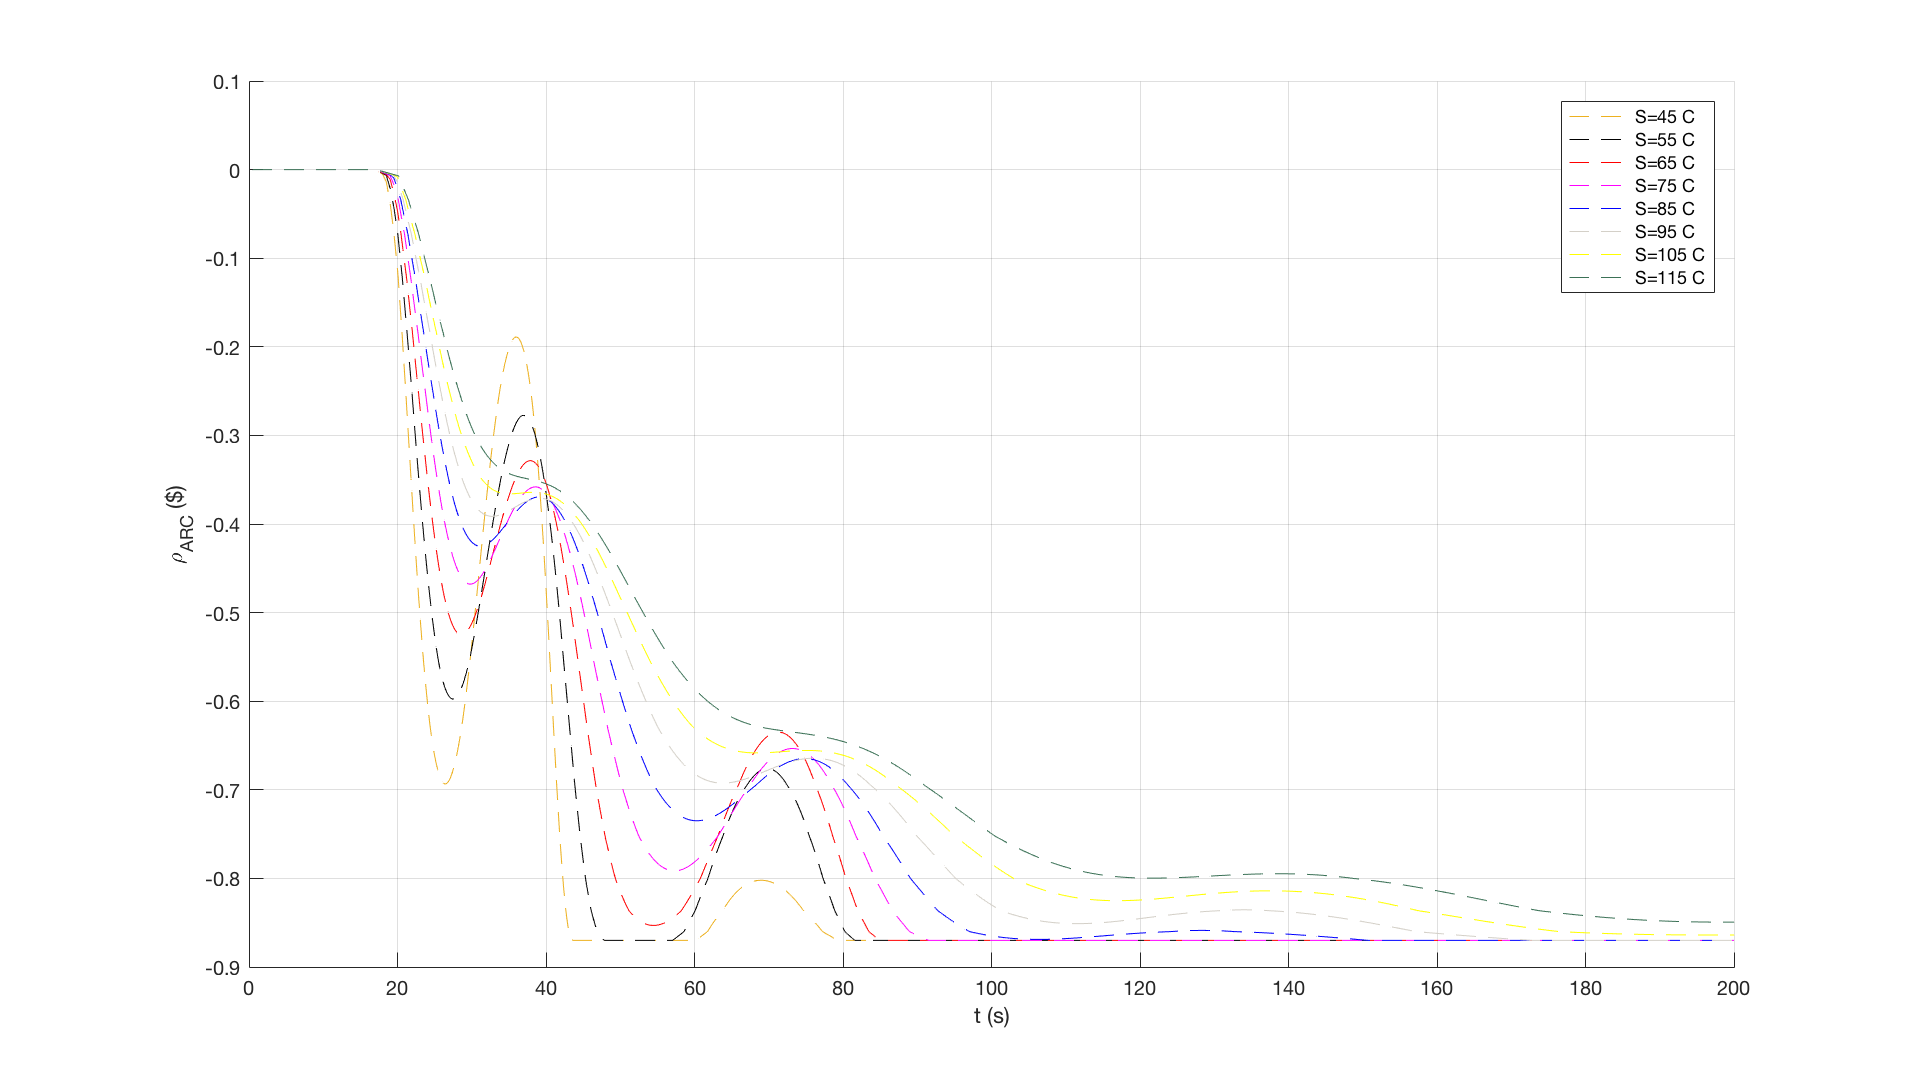
\includegraphics[width=18cm]{rho_ARC_withS}
\centering
\caption{Reactivity injected by the ARC system into the oxide ABR during the ULOF transient with increasing actuation span, $S$. $w=\$0.87$ and $\Delta T_{act}=10$ C.}
\label{fig:rho_ARC_withS}
\end{figure}

By increasing $S$, essentially the sensitivity of the ARC system is being decreased by distributing a fixed amount of reactivity worth over a greater span in actuation temperature.
Over the range of cases examined in Figure \ref{fig:rho_ARC_withS}, the average value of $\frac{d\rho_{ARC}}{dT_{act}}$ decreases from $1.9$ \cent/C to $0.8$ \cent/C, which, roughly speaking, means that the ARC system is only 40\% as sensitive in the case with $S=115$ C as compared to the case when $S=45$ C.
This seems to indicate that a method of avoiding oscillations is to decrease the sensitivity of the ARC system to changes in coolant temperature.
Another potential method of decreasing the system sensitivity to coolant temperature changes is by reducing the heat transfer ability of the upper reservoir.
By making the heat transfer from the coolant to the upper reservoir slower, sudden coolant temperature changes will not be communicated to the reservoir as quickly, and oscillating behaviors are less likely to form. 
Figure \ref{fig:rho_ARC_withTau} shows this principle for the oxide ABR with an ARC system installed with $S=65$ C, $w=\$0.87$, and $\Delta T_{act} = 10$ C.
The heat transfer to the upper reservoir is artificially retarded by increasing the value of $\tau$ supplied to the variable-lag-compensator which implements the reactivity feedback of the ARC system. 

\begin{figure}[h!]
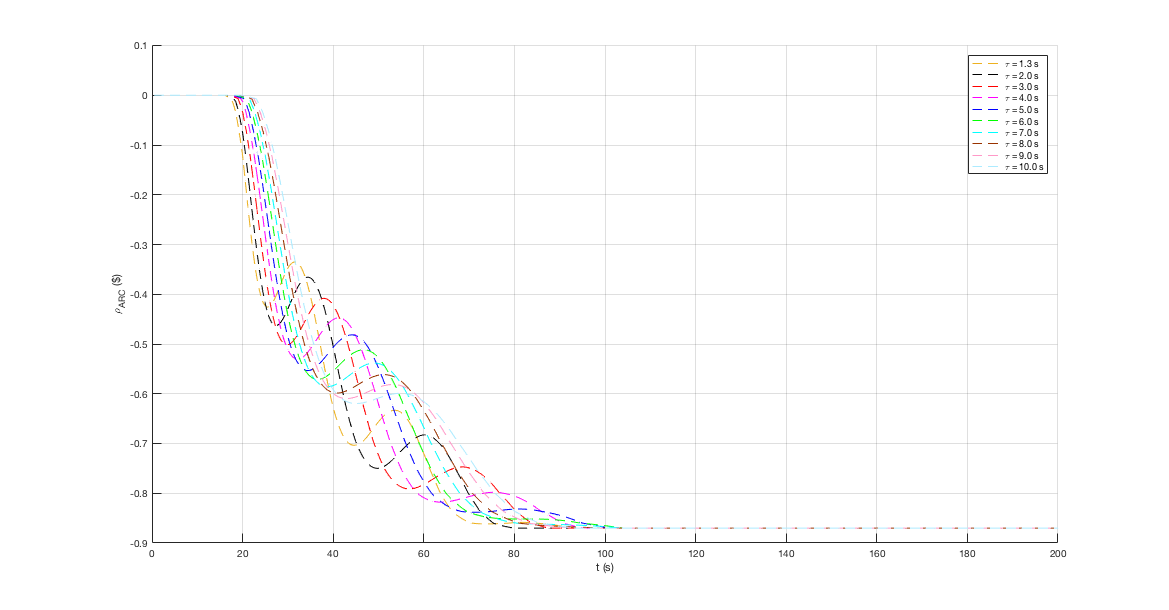
\includegraphics[width=18cm]{rho_ARC_withTau}
\centering
\caption{Reactivity injected by the ARC system into the oxide ABR during the ULOF transient with increasing heat transfer resistance from coolant to upper reservoir. $w=\$0.87$, $S=65$ C, and $\Delta T_{act}=10$ C.}
\label{fig:rho_ARC_withTau}
\end{figure}

Figure \ref{fig:rho_ARC_withTau} shows a very similar situation to Figure \ref{fig:rho_ARC_withS}, where increasing values of $\tau$ smooth out the oscillations in ARC reactivity.
This indicates that increasing $S$ and increasing $\tau$ have the same impact of making the ARC system less sensitive, and thus smoothing out oscillations.
Once again, the smoothed ARC reactivity oscillations do not necessarily translate to a smoothed temperature response, as there still exists a mismatch between the different reactivity components, as was the case for the study with increasing $S$ in section \ref{sec:increasingS}.
However, with increasing $\tau$, the speed and number of temperature oscillations is reduced.

%%%%%%%%%%%%%%%%%%%%%%%%%%%%%%%%%%%%%%%%%%%%%%%%%%%%%%%%%%%%%%%%%%%%%%%
\section{Components of the time constant $\tau$}

Even though the results shown in Section \ref{sec:tau} indicate that having a larger value of $\tau$ is better for reducing oscillatory behavior, much work has been done previously to show that an increased delay to communicate the coolant outlet temperature leads to worse oscillations \cite{ARC_Annals}.
Additionally, significant effort has been expended to achieve the smallest value of $\tau$ possible, in support of the hypothesis that a smaller $\tau$ reduces the possibility of oscillatory behavior \cite{MalwinaReport}.
This section aims to clarify how $\tau$ impacts the response of the ARC system and its role in triggering oscillatory behavior.

As outlined by Qvist et. al in \cite{ARC_Annals}, there are multiple different physical mechanisms which contribute to the delay in communicating a core temperature increase to the ARC upper reservoir.
These can be broadly split into two categories which have differing impacts on ARC system response.
The first is made up of components which cause a delay in temperature communication between the temperature in the core being brought up to the axial level of the upper reservoir.
These consist of parameters such as the coolant velocity, the presence of thermal inertia between the core and upper reservoir, and the distance between the core and upper reservoir.
The second is made up of components which cause a delay in temperature communication between the coolant fluid washing over the upper reservoir and the expander fluid within the upper reservoir.
These consist of parameters such as the heat transfer coefficient to the upper reservoir, the heat transfer area, and the thermal conductivity of the upper reservoir structure.
Both of these combine to form the total time delay for the ARC system as $\tau = \tau_{conv} + \tau_{ht}$, where $\tau_{conv}$ is the time delay due to the convection of fluid from core to reservoir and $\tau_{ht}$ is the delay due to the heat transfer from the fluid washing over the upper reservoir to the expander fluid within the upper reservoir.
In actuality, what has been studied through CFD analysis by Gradecka et. al in \cite{MalwinaReport} was $\tau_{ht}$, although it was never explicitly referred to as such.
This is the same parameter that was varied in Section \ref{sec:tau} above.

So far it has been assumed that reducing the overall $\tau$ will lead the system away from oscillatory behavior, but in fact it was shown in Section \ref{sec:tau} that \textit{increasing} $\tau_{ht}$ actually leads to damped oscillations.
Furthermore, the explanation for this behavior is obvious.
If a simple sine wave is sent into a lag-compensator, the output wave will be smaller in magnitude because the time delay never allows for the output wave to reach the full magnitude of the input.
Because the heat transfer to the ARC system behaves the same way, increasing the time constant for heat transfer will only further dampen the input wave (i.e. the coolant temperature).
Therefore, to avoid oscillations, we actually would like very poor heat transfer from the coolant to the expander fluid. 
In the limit of infinitely high thermal resistance (and thus abysmal heat transfer), for certain there will be no oscillations, as the expander fluid will never feel the impact of the increasing coolant temperature. 
In the opposite limit, every single minute change in coolant temperature will have an immediate impact on core reactivity, making the ARC system very tightly coupled and potentially unstable.

To reduce the possibility of oscillations, what we actually want to minimize is $\tau_{conv}$. 
It was shown by Qvist et. al in \cite{ARC_Annals} that increasing the mass of steel between the core and upper reservoir (i.e. increasing $\tau_{conv}$ by adding additional thermal inertia) is able to induce oscillations in the ULOF response of a core equipped with an ARC system. 
By minimizing the time that it takes to convect a core temperature increase to the level of the upper reservoir, the ARC feedback is turned into more of a prompt feedback, more similar in speed to a radial expansion feedback and less similar to a CRDL feedback, which avoids any constructive or destructive interference that the ARC reactivity may have with the CRDL feedback.

Another method of avoiding oscillations is shown in Figure \ref{fig:rho_ARC_withD}, where the axial distance between the top of the upper blanket fuel and the midpoint of the ARC upper reservoir (this parameter is referred to as D) is systematically reduced.
This is done by varying the axial position at which the coolant temperature is sampled within the SAS calculations.
Using this method does not change the position at which the ARC reservoir thermal inertia or pressure drop is felt, but only artificially alters the distance that a temperature from the active core must be convected before heating up the upper reservoir, reducing $\tau_{conv}$ while leaving $\tau_{ht}$ unaltered.

\begin{figure}[h!]
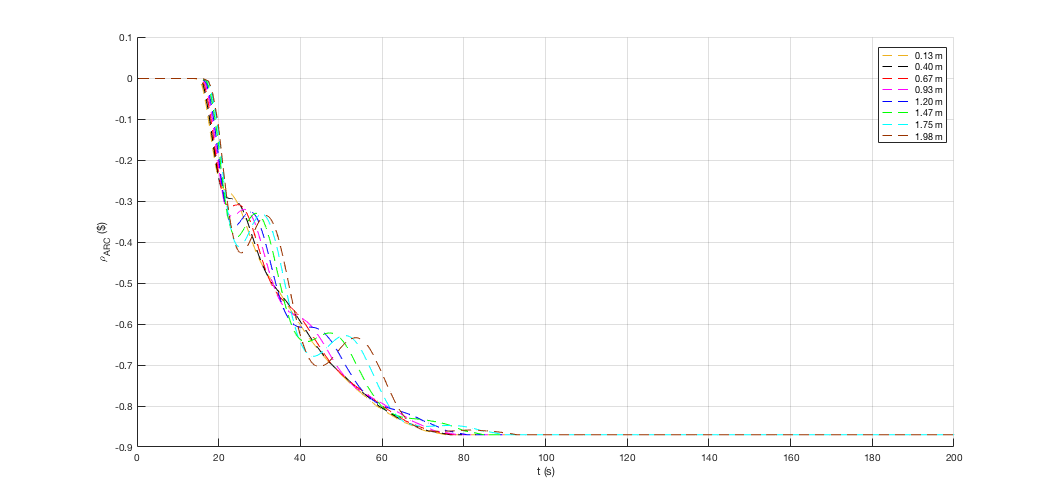
\includegraphics[width=18cm]{rho_ARC_withD}
\centering
\caption{Reactivity injected by the ARC system in the early phase of the ULOF with varying distances between the ARC upper reservoir and the top of the upper blanket fuel. $w=\$0.87$, $S=65$ C, and $\Delta T_{act}=10$ C.}
\label{fig:rho_ARC_withD}
\end{figure}

In agreement with the results in \cite{ARC_Annals}, decreasing $\tau_{conv}$ by reducing D greatly reduces the magnitude of the reactivity oscillations seen in the early ULOF phase.
This essentially has the same impact on reactivity as an increase in $\tau_{ht}$.
Furthermore, as shown in Figure \ref{fig:tempWithD}, the coolant temperature oscillations can actually be essentially eliminated by reducing D far enough, whereas the temperature oscillations never fully went away by increasing $\tau_{ht}$.
Although practical limitations such as the gas plenum length, natural circulation considerations, shielding requirements, and over-pressurization of the ARC reservoir may not allow for a physical design with such a low value for D, the trend is clear that it is beneficial to reduce D in order to avoid ARC-induced oscillations.

\begin{figure}[h!]
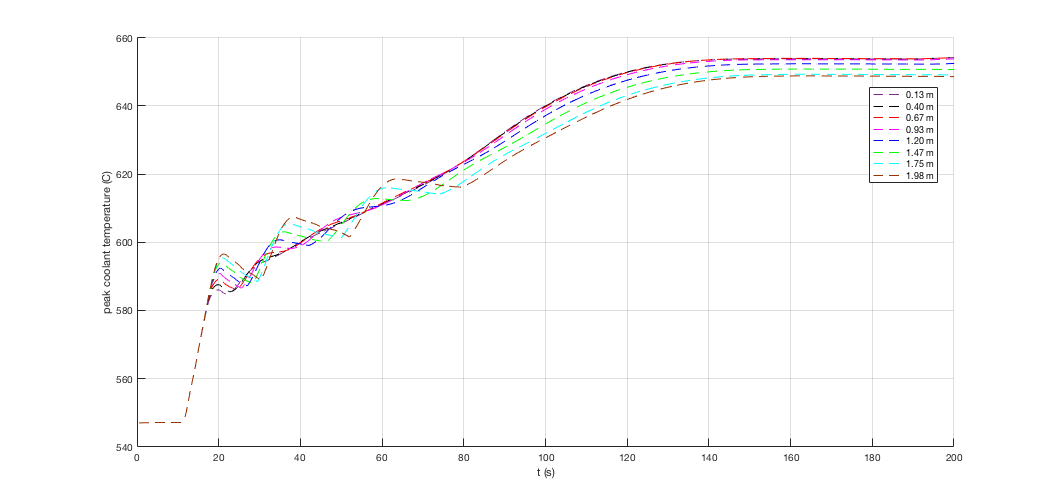
\includegraphics[width=18cm]{tempWithD}
\centering
\caption{Peak coolant temperatures in the early phase of the ULOF with varying distances between the ARC upper reservoir and the top of the upper blanket fuel, effectively changing $\tau_{conv}$. $w=\$0.87$, $S=65$ C, and $\Delta T_{act}=10$ C.}
\label{fig:tempWithD}
\end{figure}

So in order to avoid oscillations in the ARC system response, the value for the overall $\tau$ is not so important.
What is more important is to have an appropriate $\tau_{ht}$ while having a low $\tau_{conv}$.
Clearly an optimal ARC design should not have too high of a thermal resistance, as then the ARC system will not significantly contribute to arresting the transient, but a balance must be struck so that the system provides the desired negative feedback while not being overly sensitive.
Additionally, placing the upper reservoir immediately above the top of the core may not be possible due to shielding and overpressure concerns, but a balance should be achieved where $\tau_{conv}$ can be low while still allowing for other engineering constraints to be satisfied.

%%%%%%%%%%%%%%%%%%%%%%%%%%%%%%%%%%%%%%%%%%%%%%%%%%%%%%%%%%%%%%%%%%%%%%%
\section{Conclusions}

A couple of different types of oscillations are seen to occur in during the transient following a ULOF event in the oxide ABR core equipped with an ARC system.
The first type occurs following the transition from forced to natural circulation within the core.
These oscillations are larger in magnitude but slower, and are very insensitive to the design of the ARC system due to the ARC system already being fully actuated by the time that they occur.
Although it is feasible that an ARC system may be able to reduce this oscillation type in another core, essentially the pump design for the oxide ABR does not allow for any benefits to be gained.

The second type of oscillations occur early in the transient when flowrates are rapidly dropping off.
It was shown that these oscillations occur due to the reactivity from the ARC system being injected too strongly.
Two methods of reducing the reactivity oscillations were devised, namely increasing $S$ and increasing $\tau$. 
While both of these methods were able to reduce and eliminate the oscillations seen in the ARC reactivity component, neither were able to completely eliminate the resulting temperature oscillations, which are still present due to varying actuation rates between the different reactivity components.
Even though these temperature oscillations are not completely removed, the presence of the ARC system still provides great benefits to the core's ULOF response, as asymptotic temperatures are consistently brought down by over 100 C.
Additionally, these early oscillations occur at low power, are smaller than the other oscillations induced by the flow transition, and end quickly without sustained damping.
Therefore, the response of the core to the ULOF accident is deemed satisfactory.

In investigating the behavior of the core to the ULOF, it was noted that increasing $\tau$ had a beneficial impact, whereas before it was always assumed that increasing $\tau$ has a detrimental impact.
This led to a reexamination of $\tau$, and the suggestion to split up the time lag response into two time delays with different impacts, $\tau_{ht}$ and $\tau_{conv}$.
It is demonstrated that increasing $\tau_{ht}$ actually has a beneficial impact on damping oscillatory behavior.
Furthermore, it is argued that $\tau_{conv}$ is the parameter which should be decreased to avoid oscillations.
In an optimal design, a balance must be struck in the choice of $\tau_{ht}$ and $\tau_{conv}$ so that engineering constraints can be satisfied while a desired beneficial impact from ARC system inclusion is seen.

%%%%%%%%%%%%%%%%%%%%%%%%%%%%%%%%%%%%%%%%%%%%%%%%%%%%%%%%%%%%%%%%%%%%%%%
\begin{thebibliography}{9}

\bibitem{2017ANSWinter_ARC}
C. Keckler, S. Qvist, T. Fanning, M. Fratoni, E. Greenspan. "SAS4A/SASSYS-1 Simulation of ARC System in Oxide ABR for Improved Safety Margin," ANS Winter Conference, Washington DC, 2017.

\bibitem{ARC_Annals}
S. Qvist, C. Hellesen, M Gradecka, A Dubberley, T. Fanning, E. Greenspan, "Tailoring the response of Autonomous Reactivity Control (ARC) systems," Annals of Nuclear Energy (2016).

\bibitem{MalwinaReport}
M. Gradecka, S. Qvist, E. Greenspan, "High fidelity simulation of ARC systems," Summary of Task \#2 for DOE NEUP Project 15-8251.

\end{thebibliography}

\end{document}